\documentclass[border=5pt]{standalone}
\usepackage{pgfplots}
\usetikzlibrary{calc}
\pgfplotsset{compat=1.11}
\begin{document}
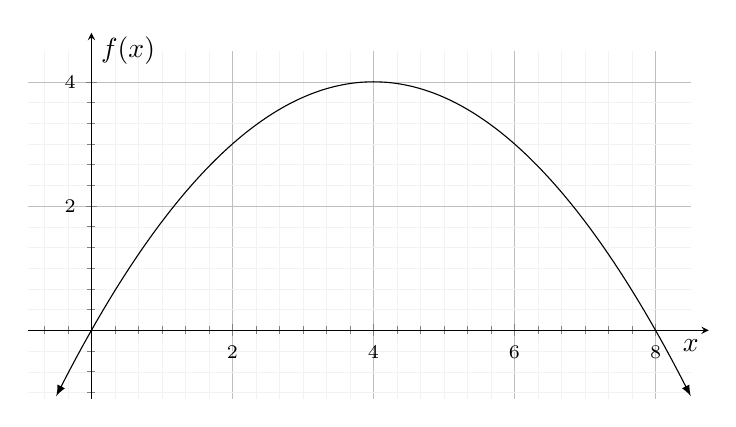
\begin{tikzpicture}
    \begin{axis}[
      width=10cm,
      height=6cm,
      xmin=-.9,
      xmax=8.5,
      ymin=-1.1,
      ymax=4.5,
      %
        axis line style={
          very thin,
            latex-latex,
            shorten >=-12.5pt,
            shorten >=-6.5pt,
        },
        axis lines=middle,
        xlabel style={at={(ticklabel* cs:1)}, anchor=north},
        ylabel style={at={(ticklabel* cs:1)}, anchor= west},
        %
        ticklabel style={font=\scriptsize},
        xlabel=$x$,
        ylabel=$f(x)$,
        %
        grid=both,
        grid style={line width=.1pt, draw=gray!10},
        major grid style={line width=.2pt,draw=gray!50},
        minor tick num=5
    ]
    \addplot[latex-latex, samples=51,smooth,domain=-.5:8.5] {-x^2/4 + 2*x};

        % %P = (25000, 625000) is a point on the parabola. The slope of the tangent line at P
        % %is -30. An equation for the tangent line at P is y = -30x + 1,375,000.
        % \coordinate (P) at (25000, 625000);
        % \coordinate (Q) at (137500/3, 0);

    \end{axis}

    %A "pin" is drawn to the parabola.
    % \draw[draw=gray, shorten <=1mm, shorten >=1mm] (P) -- ($(P)!0.75cm!90:(Q)$);
    % \node[anchor=west, inner sep=0, font=\footnotesize] at ($(P)!0.75cm!90:(Q)$){$y=P(x)$};

\end{tikzpicture}
\end{document}
